\section{Context aware models of classification}

The standard approach, showed in Picture \ref{camc1}, when dealing with \textbf{pattern recognition} problems is to;

\begin{enumerate}
    \item \textbf{Pre-process} our data;
    \item \textbf{Extract} some useful \textbf{features};
    \item Perform the \textbf{classification}.
\end{enumerate}

\begin{figure}[h!]
    \centering
    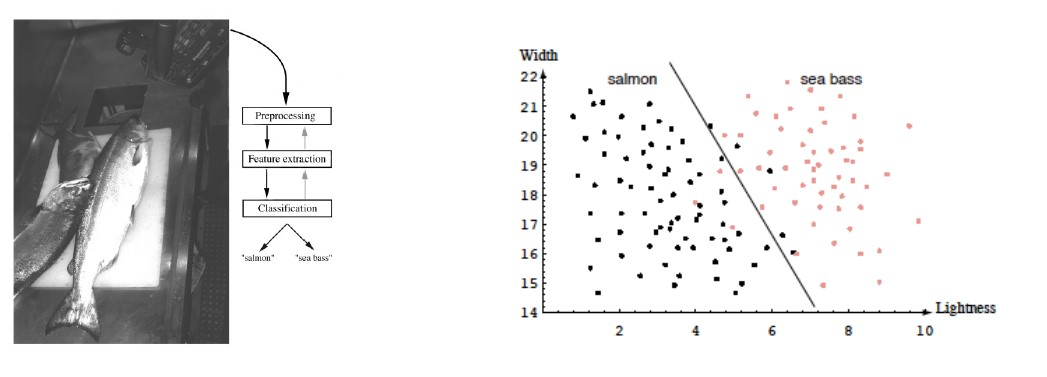
\includegraphics[scale = 1.4]{img/camc1.jpg}
    \label{camc1}
    \caption{Standard approach}
\end{figure}

However, there are some situations in which the features are ambiguous, or do not help.

\begin{figure}[h!]
    \centering
    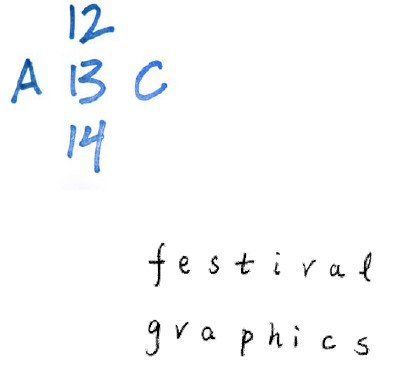
\includegraphics[scale = 1.4]{img/camc2.jpg}
    \label{camc2}
    \caption{Contextual information}
\end{figure}

For example, as showed in \ref{camc2}, we need to exploit contextual information in order to classify a digit/letter, or to pronounce a given letter or to infer the char in a sentence.

\subsection{The consistent labeling problem}
A \textbf{labeling problem} involves:

\begin{enumerate}
    \item A set of $n$ \textbf{objects} $B = {b_1, b_2, .., b_n}$;
    \item A set of $m$ \textbf{labels} $\Lambda = {1, 2, .., m}$
\end{enumerate}

, and the \textbf{goal} is to \textbf{label each object} of $B$ with a label of $\Lambda$. To this end, two sources of information are exploited:

\begin{itemize}
    \item \textbf{Local measurements}, which capture the \textbf{salient features} of each object viewed in isolation;
    \item \textbf{Contextual information}, expressed in term of a \textbf{real-valued matrix of compatibility coefficients} $R = {r_{ij}(\lambda, \mu)}$, where $r_{ij}(\lambda, \mu)$ measures the strength of compatibility between the two hypotheses :
    \begin{enumerate}
        \item $b_i$ is labeled $\lambda$;
        \item $b_j$ is labeled $\mu$.
    \end{enumerate}
    An important property is that these \textbf{compatibility coefficients} can be \textbf{learned} from \textbf{data}, and the matrix $R$ contains probability distributions.
\end{itemize}

Initially, the situation is the following:

\begin{itemize}
    \item $0 \leq p_i(\lambda) \leq 1$, $\forall \lambda \in \Lambda$;
    \item $\sum_{\lambda \in \Lambda} p_i(\lambda) = 1$.
\end{itemize}

, i.e. each object $b_i$ is characterized by a probability ditribution over the space of all the labels.

\subsection{Relaxation labeling processes}

In a classic 1976 paper, Rosenfeld, Hummel and Zucker introduced the following \textbf{update rule} (assuming a non-negative compatibility matrix):

\begin{equation}\label{eq:rel_lab}
    p_i^{(t+1)}(\lambda) = \frac{p_i^{(t)}(\lambda) q_i^{(t)}(\lambda)}{\sum_{\mu} p_i^{(t)}(\mu) q_i^{(t)}(\mu)}
\end{equation}

, where 

$$
q_i^{(t)}(\lambda) = \sum_j \sum_{\mu} r_{ij}(\lambda, \mu) p_j^{(t)} (\mu)
$$

quantifies the \textbf{support} that \textbf{context} gives at time $t$ to the hypothesis "$b_i$ is labeled with label $\lambda$".

Notice that in \ref{eq:rel_lab}, if both $p_i^{(t)}(\lambda)$ and $q_i^{(t)}(\lambda)$ assume \textbf{high value}, then $ p_i^{(t+1)}(\lambda)$ \textbf{increases}, whereas if they assume \textbf{small values}, $p_i^{(t+1)}(\lambda)$ \textbf{decreases}. Notice that the \textbf{denominator} represents a \textbf{normalization factor}, since we recall that the matrix is a probability distribution, so the elements must sum up to 1. 

This rule is used in order to make the \textbf{initial matrix} aware of the \textbf{contextual information}, and since their introduction in the mid-70's, relaxation labeling algorithms have found \textbf{applications} in virtually all problems in \textbf{CV} and \textbf{pattern recognition} (e.g. region-based segmentation, graph matching, handwritten interpretation etc..). Moreover, intriguing \textbf{similarities} exist between \textbf{relaxation labeling processes} and certain mechanisms in the \textbf{early stage of biological visual systems}.

\subsection{Hummel and Zucker's consistency}
In 1983, Hummel and Zucker developed an elegant theory of \textbf{consistency}
in labeling problem. By analogy with the unambiguous case, which is easily understood, they define a \textbf{weighted labeling assignment} $p$ \textbf{consistent} if:

\begin{equation}
    \sum_{\lambda} p_i(\lambda) q_i(\lambda) \geq \sum_{\lambda} v_i(\lambda) q_i(\lambda)
\end{equation}

for all labeling assignments $v$.

This basically represents a \textbf{generalization} of the \textbf{classical} (Boolean) \textbf{constraint satisfaction problems}, since in a general CSP we want to assign the vertices some labels according to some logical constraints. In this case, we have two differences:

\begin{enumerate}
    \item The \textbf{constraints} are \textbf{soft}, not logical;
    \item The \textbf{labeling} we use are not hard, but \textbf{probabilistic}. In this sense, each vertex is not assigned a single label, but a probability distribution over all the possible labels.
\end{enumerate}

\subsection{Relaxation labeling as a non-cooperative game}
As observed by Miller and Zucker (1991) the consistent labeling problem is equivalent to a non-cooperative (polymatrix) game. In such formulation we have:

\begin{itemize}
    \item Players = Objects;
    \item Pure strategies = Labels;
    \item Mixed strategies = Weighted labeling assignments;
    \item Payoffs = Compatibility coefficients,
\end{itemize}

and the concept of \textbf{Nash equilibrium} can be put in one-to-one correspondence to the one of \textbf{consistent labeling}.

Further, the Rosenfeld-Hummel-Zucker update rule corresponds to discrete-time
multi-population replicator dynamics.

\subsection{Application to semi-supervised learning}
Differently from a classical supervised learning, in which all the examples of the dataset are associated with a label, in the case of \textbf{semi-supervised learning} only a \textbf{fraction} of the dataset is \textbf{labeled}, so the goal is to use the labeled objects to classify the unlabeled ones.

\begin{figure}[h!]
    \centering
    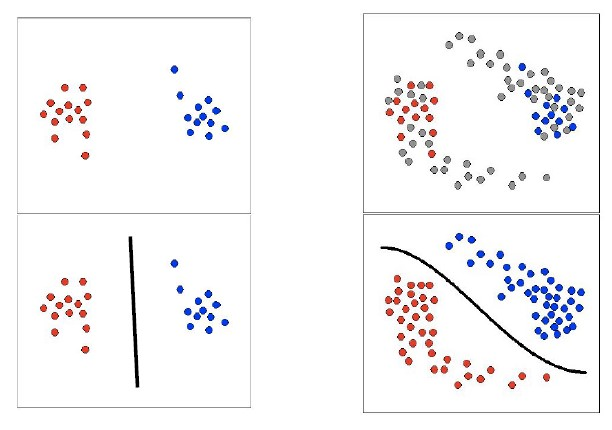
\includegraphics[scale = 1.4]{img/camc4.jpg}
    \label{camc4}
    \caption{Semi-supervised learning}
\end{figure}

In this sense, the final model will take into account both labeled and unlabeled data points.

\subsection{Graph transduction}
The problem of \textbf{graph transduction} can be formulated as follows: given a set of data points grouped into:

\begin{itemize}
    \item \textbf{Labeled} data ${(x_1, y_1), (x_2, y_2), .., (x_l, y_l)}$ ;
    \item \textbf{Unlabeled} data $x_{l+1}, .., x_n$, with $l \ll n$
\end{itemize}

, we can express a graph $G = (V,E)$ where:

\begin{itemize}
    \item $V$ are the \textbf{nodes} representing \textbf{labeled} and \textbf{unlabeled} points;
    \item $E$ are the \textbf{edges} between nodes \textbf{weighted} by the similarity between the corresponding pairs of points.
\end{itemize}

Then, the goal is to \textbf{propagate} the information \textbf{available} at the \textbf{labeled nodes} \textbf{to} \textbf{unlabeled ones} in a “consistent” way. In this case consistent means that the data form \textbf{distinct clusters}, and two points in the same cluster are expected to be in the same class. (CSP problem!)

A simple case of graph transduction in which the graph $G$ is an unweighted undirected graph:

\begin{itemize}
    \item An edge denotes perfect similarity between points;
    \item The adjacency matrix of $G$ is a 0/1 matrix.
\end{itemize}

An important \textbf{property} of this problem is that it can be formulated as a \textbf{non-cooperative game}. Given a weighted graph $G = (V,E,w)$, the graph transduction game (GTG) is as follow:

\begin{itemize}
    \item Players = Objects;
    \item Pure strategies = Labels;
    \item Mixed strategies = Weighted labeling assignments;
    \item Payoffs = Compatibility coefficients
\end{itemize}

The transduction game is in fact played among the unlabeled players to choose
their memberships. In this sense, the concept of \textbf{Nash equilibrium} can be put into one-to-one correspondence with \textbf{consistent labeling} of nodes, and it can be solved using\textbf{ standard relaxation labeling / replicator dynamics}. Moreover, the framework can cope with symmetric, negative and asymmetric similarities and category-level similarities.

\subsubsection{Word sense disambiguation}
\textbf{WSD} is the task of \textbf{identifying} the \textbf{intended meaning of a word based on the context in which it appears}. It has been studied since the beginning of NLP and also today is a central topic of this discipline, since it is used in applications like text understanding, machine translation, opinion mining, sentiment analysis and information extraction.

The WSD problem can be formulated in \textbf{game-theoretic terms modeling}:

\begin{itemize}
    \item The players of the games as the words to be disambiguated;
    \item The strategies of the games as the senses of each word;
    \item The payoff matrices of each game as a sense similarity function;
    \item The interactions among the players as a weighted graph.
\end{itemize}

In this case the \textbf{Nash equilibrium} correspond to \textbf{consistent word-sense assignments}!

\begin{itemize}
    \item \textbf{Word-level similarities}: proportional to strength of co-occurrence between words;
    \item \textbf{Sense-level similarities}: computed using WordNet / BabelNet ontologies.
\end{itemize}

Picture \ref{camc5} shows an example of a sentence, while \ref{camc6_9} shows the iterations of the solution of the WSD problem.

\begin{figure}[h!]
    \centering
    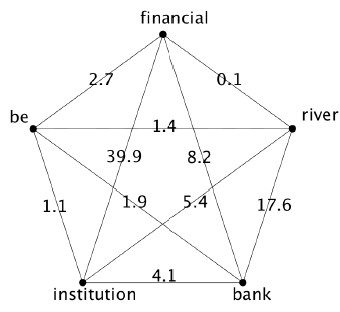
\includegraphics[scale = 1.4]{img/camc5.jpg}
    \label{camc5}
    \caption{Example of graph for the graph-transduction problem}
\end{figure}

\begin{figure}[h!]
    \centering
    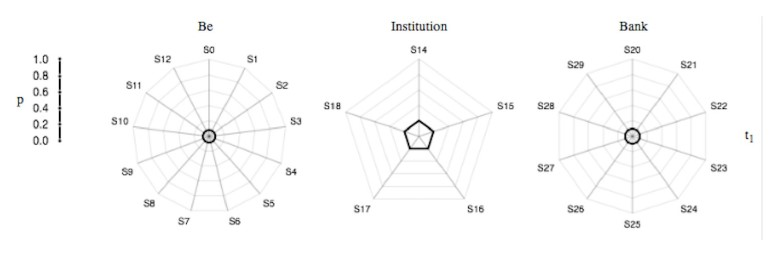
\includegraphics[scale = 1.4]{img/camc6.jpg}
    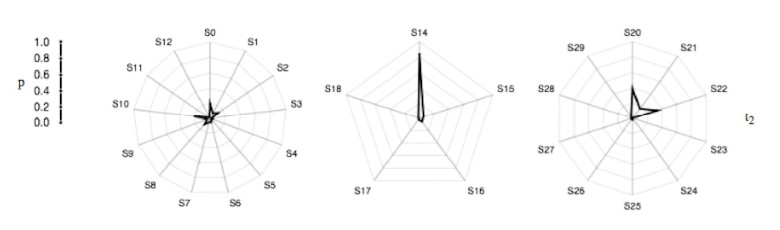
\includegraphics[scale = 1.4]{img/camc7.jpg}
    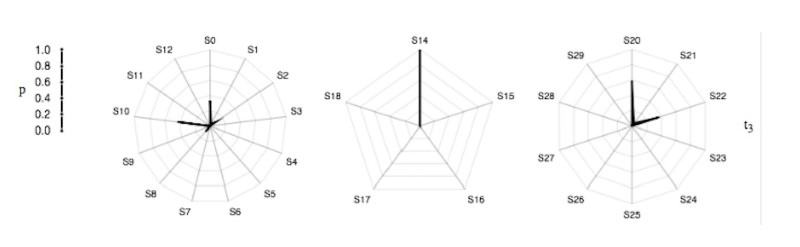
\includegraphics[scale = 1.4]{img/camc8.jpg}
    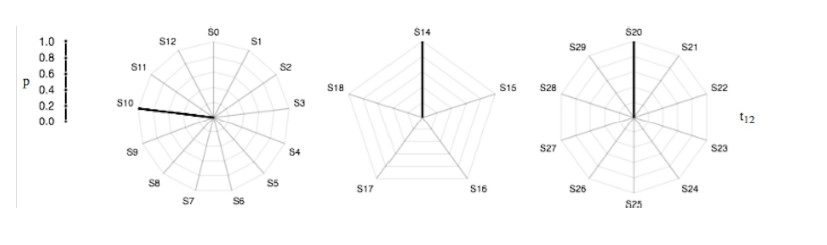
\includegraphics[scale = 1.4]{img/camc9.jpg}
    \label{camc6_9}
    \caption{Example of WSD game dynamics}
\end{figure}

As we can see, initially, each of the senses of the words have the same probability, and then these probabilities are updated as the algorithm proceeds the execution. 

\subsubsection{The "protein function prediction" game}
\textbf{Network-based methods} for the \textbf{automatic prediction of protein functions} can greatly benefit from exploiting both the similarity between proteins and the similarity between functional classes. \textbf{Hume’s principle} states that \textbf{similar proteins} should have \textbf{similar functionalities}.

We envisage a (non-cooperative) game where:

\begin{itemize}
    \item Players = proteins;
    \item Strategies = functional classes;
    \item Payoff function = combination of protein- and function-level similarities.
\end{itemize}

The \textbf{Nash equilibrium} turns out to provide \textbf{consistent functional labelings of proteins}.

\subsection{Metric learning: triplet loss}
We now present a system, called \textbf{FaceNet}, that directly learns a \textbf{mapping} from \textbf{face images} to a \textbf{compact Euclidean space} where \textbf{distances} directly \textbf{correspond} to a \textbf{measure of face similarity}. Once this space has been produced, tasks such as face recognition, verification and clustering can be easily implemented using standard techniques with FaceNet embeddings as feature vectors.

The problem of embedding an image into an Euclidean space is represented in Picture \ref{camc10}.

\begin{figure}[h!]
    \centering
    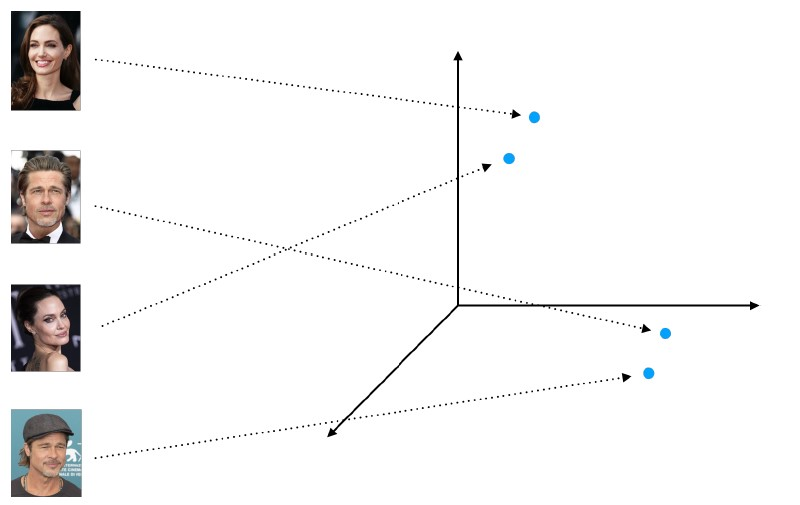
\includegraphics[scale = 1.4]{img/camc10.jpg}
    \label{camc10}
    \caption{Embedding an image into an Euclidean space}
\end{figure}

\subsubsection{The triplet loss}
The concept on which the embedding is based is the so-called \textbf{triplet loss}. The idea is to take \textbf{3 instances} from the training set: an \textbf{anchor}, a \textbf{negative instance} (with different label w.r.t. the anchor) and a \textbf{positive instance} (with the same label of the anchor). Thus, the goal of the embedding is to:

\begin{itemize}
    \item \textbf{Minimize} the \textbf{distance} between the \textbf{anchor} and the \textbf{positive} example;
    \item \textbf{Maximize} the \textbf{distance} between the \textbf{anchor} and the \textbf{negative} example.
\end{itemize}

A visual representation of the relationships between anchor, negative and positive examples is provided in Picture \ref{camc11_12}.

\begin{figure}[h!]
    \centering
    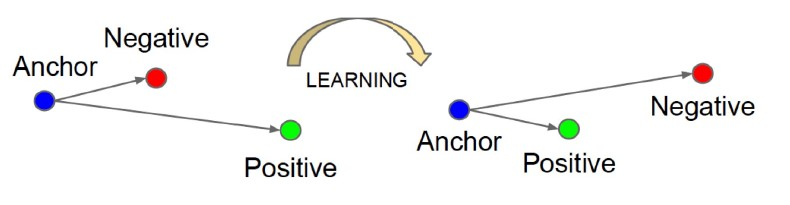
\includegraphics[scale = 1.2]{img/camc11.jpg}
    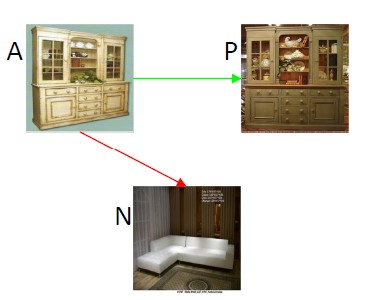
\includegraphics[scale = 1.5]{img/camc12.jpg}
    \label{camc11_12}
    \caption{Anchor, negative and positive examples}
\end{figure}

Picture \ref{camc13} shows the \textbf{goal} of the embedding: the \textbf{distance} in the Euclidean space between the embedding representation of the anchor, negative and positive examples must be \textbf{minimized}.

\begin{figure}[h!]
    \centering
    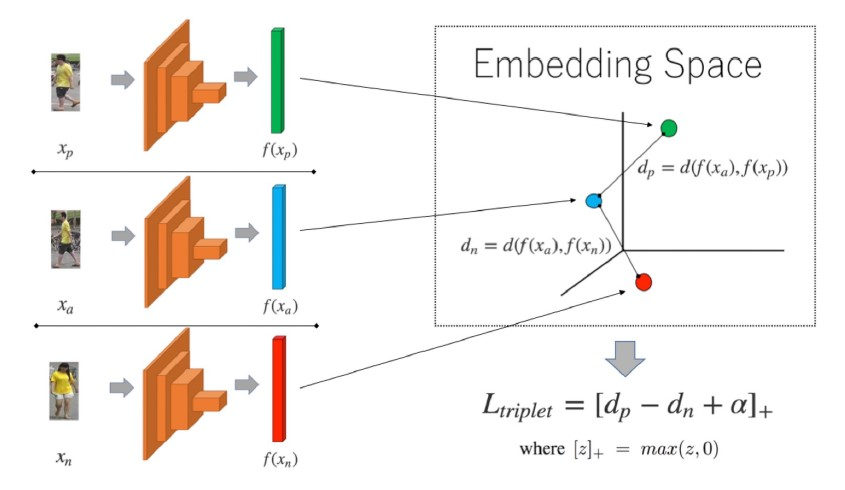
\includegraphics[scale = 1.4]{img/camc13.jpg}
    \label{camc13}
    \caption{Triplet loss}
\end{figure}

In particular, the Picture shows the exact \textbf{loss} to be minimized. As we can see the loss is defined as 

$$
L_{\text{triplet}} = \max(d_p - d_n + \alpha, 0)
$$

, which means that:

\begin{itemize}
    \item If $d_p - d_n + \alpha \leq 0$, then the loss is equal to 0, as we desire;
    \item Otherwise, the loss has value $d_p - d_n + \alpha > 0$.
\end{itemize}

\subsubsection{Pipeline}
Picture \ref{camc14} shows the \textbf{pipeline} of the triplet loss computation.

\begin{figure}[h!]
    \centering
    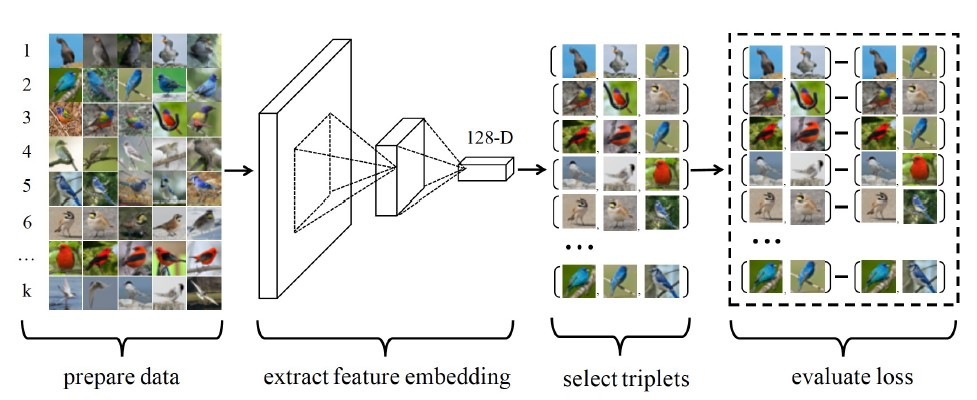
\includegraphics[scale = 1.4]{img/camc14.jpg}
    \label{camc14}
    \caption{The triplet loss pipeline}
\end{figure}

As we can see:

\begin{itemize}
    \item In the \textbf{first stage}, a \textbf{mini-batch} is sampled from the training data, which usually contains $k$ identities with several images per identity;
    \item \textbf{Deep Neural Networks} are used to \textbf{learn} a \textbf{feature embedding}, e.g. a 128-dimensions feature vector;
    \item In the \textbf{third stage}, a subset of \textbf{triplets} are selected using some \textbf{triplet selection methods};
    \item Lastly, the \textbf{loss} is evaluated using the selected triplets.
\end{itemize}

\subsubsection{The group loss}
Clearly, we can \textbf{generalize} the concept of \textbf{triplet loss} by considering \textbf{all the relations among the nodes} contained in the mini-batch, and not only considering triplets. An example of \textbf{group loss} is provided in Picture \ref{camc15}.

\begin{figure}[h!]
    \centering
    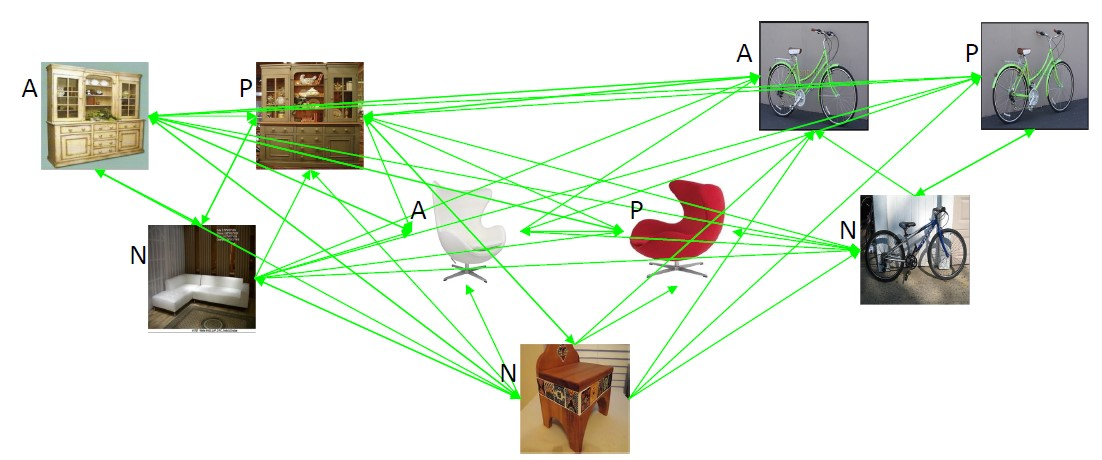
\includegraphics[scale = 1.4]{img/camc15.jpg}
    \label{camc15}
    \caption{Group loss}
\end{figure}

Picture \ref{camc16} shows the \textbf{pipeline} of this new approach.

\begin{figure}[h!]
    \centering
    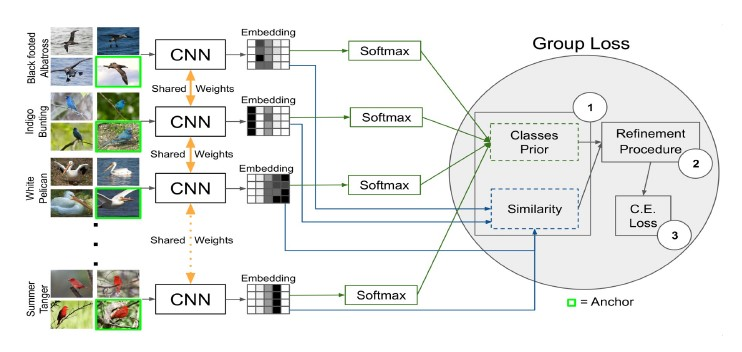
\includegraphics[scale = 1.5]{img/camc16.jpg}
    \label{camc16}
    \caption{The group loss pipeline}
\end{figure}

As we can see:

\begin{itemize}
    \item Again, \textbf{CNN's} are used to retrieve the \textbf{feature embeddings}. Notice that the different CNN's are characterized by the fact that they \textbf{share} the same set of \textbf{weights};
    \item Then, we have three steps:
    \begin{enumerate}
        \item \textbf{Initialization}: initialize X, the image-label assignment using the softmax outputs of the NN. Compute the $n \times x$ pairwise similarity matrix $W$ using the NN embeddings;
        \item \textbf{Refinement}: iteratively, refine $X$ considering the similarities between all the mini-batches images, as encoded in $W$, as well as their labeling preferences;
        \item \textbf{Loss computation}: compute the cross-entropy loss of the refined probabilities and update the weights of the NN using backpropagation.
    \end{enumerate}
\end{itemize}

As we can see, the \textbf{goal} of the \textbf{loss function} is to \textbf{refine} the \textbf{soft-labels} predicted by a neural network, using an \textbf{iterative procedure} based on the similarity between the images in the mini-batch.

Picture \ref{camc17} shows a toy \textbf{example} of the refinement procedure, where the goal is to classify sample C based on the similarity with samples A and B. 

\begin{figure}[h!]
    \centering
    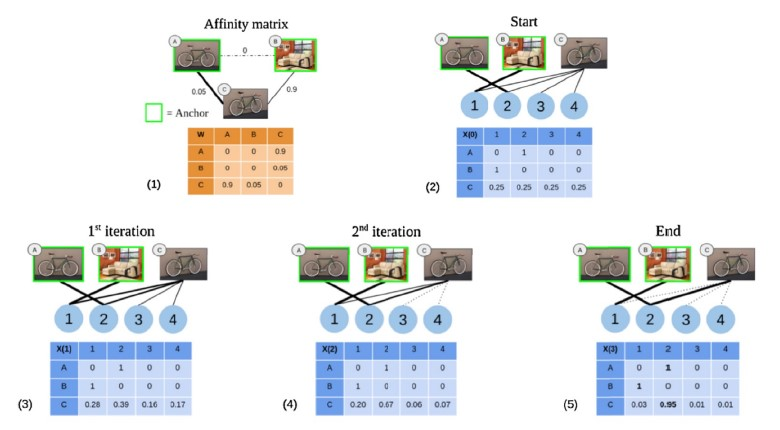
\includegraphics[scale = 1.7]{img/camc17.jpg}
    \label{camc17}
    \caption{Results}
\end{figure}

(1) The affinity matrix used to update the soft assignments. (2) The initial labeling of the matrix. (3-4) The process iteratively refines the soft assignment of the unlabeled sample C. (5) At the end of the process, sample C
gets the same label of A, (A, C) being more similar than (B, C).